% Options for packages loaded elsewhere
\PassOptionsToPackage{unicode}{hyperref}
\PassOptionsToPackage{hyphens}{url}
%
\documentclass[
]{article}
\usepackage{lmodern}
\usepackage{amssymb,amsmath}
\usepackage{ifxetex,ifluatex}
\ifnum 0\ifxetex 1\fi\ifluatex 1\fi=0 % if pdftex
  \usepackage[T1]{fontenc}
  \usepackage[utf8]{inputenc}
  \usepackage{textcomp} % provide euro and other symbols
\else % if luatex or xetex
  \usepackage{unicode-math}
  \defaultfontfeatures{Scale=MatchLowercase}
  \defaultfontfeatures[\rmfamily]{Ligatures=TeX,Scale=1}
\fi
% Use upquote if available, for straight quotes in verbatim environments
\IfFileExists{upquote.sty}{\usepackage{upquote}}{}
\IfFileExists{microtype.sty}{% use microtype if available
  \usepackage[]{microtype}
  \UseMicrotypeSet[protrusion]{basicmath} % disable protrusion for tt fonts
}{}
\makeatletter
\@ifundefined{KOMAClassName}{% if non-KOMA class
  \IfFileExists{parskip.sty}{%
    \usepackage{parskip}
  }{% else
    \setlength{\parindent}{0pt}
    \setlength{\parskip}{6pt plus 2pt minus 1pt}}
}{% if KOMA class
  \KOMAoptions{parskip=half}}
\makeatother
\usepackage{xcolor}
\IfFileExists{xurl.sty}{\usepackage{xurl}}{} % add URL line breaks if available
\IfFileExists{bookmark.sty}{\usepackage{bookmark}}{\usepackage{hyperref}}
\hypersetup{
  hidelinks,
  pdfcreator={LaTeX via pandoc}}
\urlstyle{same} % disable monospaced font for URLs
\usepackage[margin=1in]{geometry}
\usepackage{color}
\usepackage{fancyvrb}
\newcommand{\VerbBar}{|}
\newcommand{\VERB}{\Verb[commandchars=\\\{\}]}
\DefineVerbatimEnvironment{Highlighting}{Verbatim}{commandchars=\\\{\}}
% Add ',fontsize=\small' for more characters per line
\usepackage{framed}
\definecolor{shadecolor}{RGB}{248,248,248}
\newenvironment{Shaded}{\begin{snugshade}}{\end{snugshade}}
\newcommand{\AlertTok}[1]{\textcolor[rgb]{0.94,0.16,0.16}{#1}}
\newcommand{\AnnotationTok}[1]{\textcolor[rgb]{0.56,0.35,0.01}{\textbf{\textit{#1}}}}
\newcommand{\AttributeTok}[1]{\textcolor[rgb]{0.77,0.63,0.00}{#1}}
\newcommand{\BaseNTok}[1]{\textcolor[rgb]{0.00,0.00,0.81}{#1}}
\newcommand{\BuiltInTok}[1]{#1}
\newcommand{\CharTok}[1]{\textcolor[rgb]{0.31,0.60,0.02}{#1}}
\newcommand{\CommentTok}[1]{\textcolor[rgb]{0.56,0.35,0.01}{\textit{#1}}}
\newcommand{\CommentVarTok}[1]{\textcolor[rgb]{0.56,0.35,0.01}{\textbf{\textit{#1}}}}
\newcommand{\ConstantTok}[1]{\textcolor[rgb]{0.00,0.00,0.00}{#1}}
\newcommand{\ControlFlowTok}[1]{\textcolor[rgb]{0.13,0.29,0.53}{\textbf{#1}}}
\newcommand{\DataTypeTok}[1]{\textcolor[rgb]{0.13,0.29,0.53}{#1}}
\newcommand{\DecValTok}[1]{\textcolor[rgb]{0.00,0.00,0.81}{#1}}
\newcommand{\DocumentationTok}[1]{\textcolor[rgb]{0.56,0.35,0.01}{\textbf{\textit{#1}}}}
\newcommand{\ErrorTok}[1]{\textcolor[rgb]{0.64,0.00,0.00}{\textbf{#1}}}
\newcommand{\ExtensionTok}[1]{#1}
\newcommand{\FloatTok}[1]{\textcolor[rgb]{0.00,0.00,0.81}{#1}}
\newcommand{\FunctionTok}[1]{\textcolor[rgb]{0.00,0.00,0.00}{#1}}
\newcommand{\ImportTok}[1]{#1}
\newcommand{\InformationTok}[1]{\textcolor[rgb]{0.56,0.35,0.01}{\textbf{\textit{#1}}}}
\newcommand{\KeywordTok}[1]{\textcolor[rgb]{0.13,0.29,0.53}{\textbf{#1}}}
\newcommand{\NormalTok}[1]{#1}
\newcommand{\OperatorTok}[1]{\textcolor[rgb]{0.81,0.36,0.00}{\textbf{#1}}}
\newcommand{\OtherTok}[1]{\textcolor[rgb]{0.56,0.35,0.01}{#1}}
\newcommand{\PreprocessorTok}[1]{\textcolor[rgb]{0.56,0.35,0.01}{\textit{#1}}}
\newcommand{\RegionMarkerTok}[1]{#1}
\newcommand{\SpecialCharTok}[1]{\textcolor[rgb]{0.00,0.00,0.00}{#1}}
\newcommand{\SpecialStringTok}[1]{\textcolor[rgb]{0.31,0.60,0.02}{#1}}
\newcommand{\StringTok}[1]{\textcolor[rgb]{0.31,0.60,0.02}{#1}}
\newcommand{\VariableTok}[1]{\textcolor[rgb]{0.00,0.00,0.00}{#1}}
\newcommand{\VerbatimStringTok}[1]{\textcolor[rgb]{0.31,0.60,0.02}{#1}}
\newcommand{\WarningTok}[1]{\textcolor[rgb]{0.56,0.35,0.01}{\textbf{\textit{#1}}}}
\usepackage{graphicx,grffile}
\makeatletter
\def\maxwidth{\ifdim\Gin@nat@width>\linewidth\linewidth\else\Gin@nat@width\fi}
\def\maxheight{\ifdim\Gin@nat@height>\textheight\textheight\else\Gin@nat@height\fi}
\makeatother
% Scale images if necessary, so that they will not overflow the page
% margins by default, and it is still possible to overwrite the defaults
% using explicit options in \includegraphics[width, height, ...]{}
\setkeys{Gin}{width=\maxwidth,height=\maxheight,keepaspectratio}
% Set default figure placement to htbp
\makeatletter
\def\fps@figure{htbp}
\makeatother
\setlength{\emergencystretch}{3em} % prevent overfull lines
\providecommand{\tightlist}{%
  \setlength{\itemsep}{0pt}\setlength{\parskip}{0pt}}
\setcounter{secnumdepth}{-\maxdimen} % remove section numbering

\author{}
\date{\vspace{-2.5em}}

\begin{document}

\hypertarget{introduction}{%
\section{Introduction}\label{introduction}}

\hypertarget{datavis-introduction}{%
\subsection{DataVis Introduction}\label{datavis-introduction}}

Data Science is crucial for many applications in a variety of fields and
is the language of collaboration between biology, computer science,
bioinformatics, physics, and mathematics.

Goals of this course include to introduce you to the R and Rstudio, and
provide you general analytic techniques to extract knowledge, patterns,
and connections between samples and variables, and how to communicate
these in an intuitive and clear way. Some of the examples will be
expressed in the field of bioinformatics.

\hypertarget{what-is-data-science}{%
\subsubsection{What is Data Science?}\label{what-is-data-science}}

Data science is an interdisciplinary field about processes and systems
to extract knowledge or insights from data in various forms, either
structured or unstructured. It is a continuation of some of the data
analysis fields such as statistics, data mining, and predictive
analytics.

The Goals of Data Science include discovering new phenomena or trends
from data, enabling decisions based on facts derived from data, and
communicating findings from data.

Data science at its core is the heart of any scientific method, start
with observations, make hypotheses, experiment, and visualize the
results in such a way that you can make claims about the validity of the
hypothesis. These skills are applicable not only to whatever research
topic interests you, but are also some of the hottest skills you may
develop for the job market.

\hypertarget{what-youll-learn}{%
\subsubsection{What you'll learn}\label{what-youll-learn}}

Opposed to many other statistics or machine learning lectures this
course is designed to teach you the practical skills you need as a data
scientist. We will not focus on the complex math that went into
developing the high powered statistical tools, and machine learning
techniques thought in many courses. We will focus on tidy data,
visualizations, and data manipulation in R. To only then dive into the
math required to understand and interpret analysis results.

\hypertarget{our-tool}{%
\subsubsection{Our tool}\label{our-tool}}

\begin{itemize}
\tightlist
\item
  R- a language and program designed for data analytics. Not great for
  big applications, but an environment to work with data in an easy way
  based on scripts.

  \begin{itemize}
  \tightlist
  \item
    Scripting: work on the fly, define few functions and data structures
    but use existing packages to interpret your data along with your own
    intuition.
  \item
    Package developer: robust, fast code, that copes with the inherent
    problems of the language.
  \end{itemize}
\end{itemize}

\hypertarget{breakdown-of-topics}{%
\subsubsection{Breakdown of topics}\label{breakdown-of-topics}}

\begin{itemize}
\tightlist
\item
  R markdown: Notebooks that allow you to quickly publish and share your
  code informally so that you can see the results and the code that
  generated it. (This is an R markdown file)
\item
  Tidy data: standard way of structuring data for efficient memory
  storage and efficient operations
\item
  Visualization with ggplot2: flexible grammar and frame-work to
  visualize data in concise and easy ways.
\item
  Hypothesis testing and hypothesis generation: data exploration allows
  you to identify possible correlations and relationships. Hypothesis
  testing helps with identifying the validity of the hypothesis.

  \begin{itemize}
  \tightlist
  \item
    T-test, Wilcoxon, Fisher test, resampling approaches
  \end{itemize}
\item
  Predictions: Supervised learning approaches
\item
  Regression, classification, and assessing predictive power
\end{itemize}

\hypertarget{introduction-to-r-and-rstudio}{%
\subsection{Introduction to R and
Rstudio}\label{introduction-to-r-and-rstudio}}

\begin{itemize}
\tightlist
\item
  R is the language of this course. It shares some aspects with python,
  but the syntax is often unique compared to other languages. All R
  files are named with a .R extension (dot - R)\\
\item
  Rstudio is an editor, it succinctly organizes your session into 4
  windows each set up for you to do certain tasks in each window. Edit
  and write code (editor), run and execute code (console), list and name
  objects, and a window to show output in either function help, and
  plots.
\end{itemize}

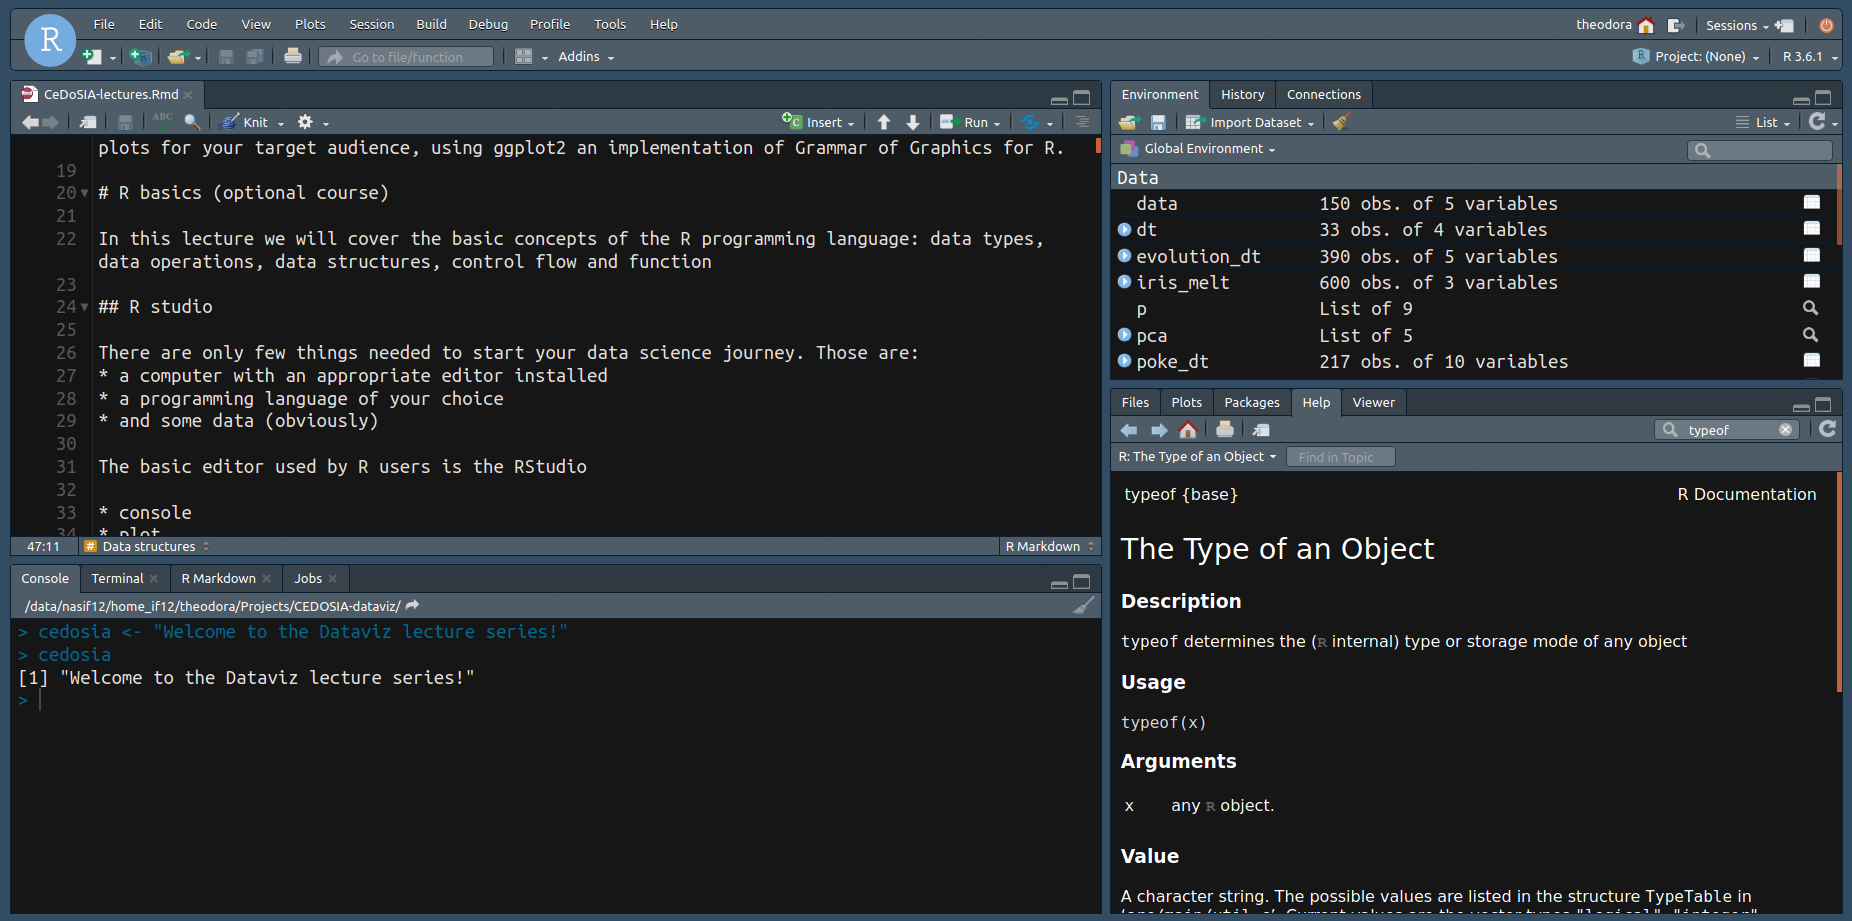
\includegraphics[width=900px]{assets/img/RStudio}

The most commonly used editor by R users is the RStudio. It consists of
the following sections such as:

\begin{itemize}
\tightlist
\item
  the main script section, for writing scripts {[}top left section{]}
  (Ctrl+1 to focus)
\item
  the console tab, for typing R commands directly {[}bottom left section
  as tab{]} (Ctrl+2 to focus)
\item
  the terminal tab, for direct access to your system shell {[}bottom
  left section{]} (Shift+Alt+T to focus)
\item
  the plot tab, where you see the last plot generated {[}bottom right
  section as tab{]}
\item
  the help tab, with useful documentation of R functions {[}bottom right
  section as tab{]} (F1 on the name of a function or Ctrl+3)
\item
  the history tab, with the list of the R commands used {[}top right
  section as tab{]}
\item
  the environment tab, with the created variables and functions loaded
  {[}top right section as tab{]}
\item
  and the packages tab, with the available/loaded R packages {[}bottom
  right section as tab{]}
\end{itemize}

Check the View menu to find out the rest of useful shortcuts!

\hypertarget{intro-to-basic-r-syntax}{%
\subsubsection{Intro to basic R syntax}\label{intro-to-basic-r-syntax}}

\begin{itemize}
\tightlist
\item
  All code is run in the console (bottom left) you can write and alter
  code directly in here or in the editor above (top left) for easier
  editing/debugging
\item
  All of your questions and issues can be investigated
  \href{https://cran.r-project.org/doc/contrib/Paradis-rdebuts_en.pdf}{Here}
\item
  R examples:

  \begin{itemize}
  \tightlist
  \item
    basic operators
  \end{itemize}

\begin{Shaded}
\begin{Highlighting}[]
\NormalTok{x <-}\StringTok{ }\DecValTok{10}
\NormalTok{x}
\end{Highlighting}
\end{Shaded}

\begin{verbatim}
## [1] 10
\end{verbatim}

\begin{Shaded}
\begin{Highlighting}[]
\NormalTok{x }\OperatorTok{+}\StringTok{ }\DecValTok{5}
\end{Highlighting}
\end{Shaded}

\begin{verbatim}
## [1] 15
\end{verbatim}

\begin{Shaded}
\begin{Highlighting}[]
\NormalTok{y <-}\StringTok{ }\NormalTok{x }\OperatorTok{+}\StringTok{ }\DecValTok{5}
\NormalTok{y}
\end{Highlighting}
\end{Shaded}

\begin{verbatim}
## [1] 15
\end{verbatim}

\begin{Shaded}
\begin{Highlighting}[]
\NormalTok{x }\OperatorTok{==}\StringTok{ }\NormalTok{y}
\end{Highlighting}
\end{Shaded}

\begin{verbatim}
## [1] FALSE
\end{verbatim}

\begin{Shaded}
\begin{Highlighting}[]
\NormalTok{x}
\end{Highlighting}
\end{Shaded}

\begin{verbatim}
## [1] 10
\end{verbatim}

  \begin{itemize}
  \tightlist
  \item
    built-in methods
  \end{itemize}

\begin{Shaded}
\begin{Highlighting}[]
\NormalTok{x <-}\StringTok{ }\KeywordTok{rnorm}\NormalTok{(}\DecValTok{10}\NormalTok{) }\CommentTok{#returns a vector of random numbers based on the normal distribution}
\KeywordTok{mean}\NormalTok{(x)}
\end{Highlighting}
\end{Shaded}

\begin{verbatim}
## [1] -0.1142763
\end{verbatim}
\item
  \textbf{?} operator\\
  \texttt{?mean} shows you information about the function you are
  calling. Look to the bottom right window.
\end{itemize}

We will introduce further details of the R language as they are needed
throughout the course and refer you to the Appendix II for a more
detailed introduction to R.

\pagebreak

\end{document}
